\documentclass{beamer}
\usepackage{amsfonts, amssymb, amsmath, amsthm, graphicx, multirow, beamerthemesplit}

\title[Bayesian Copula Modeling for Clinical Trials]{Copula Modeling for Clinical Trials}
\author{Nathan T. James, ScM}
\institute{Department of Biostatistics, Vanderbilt University}
\date{February 26, 2019}

\begin{document}
	
	\frame{\titlepage}	
%	\frame{\tableofcontents}
	
\section{Introduction}

	\begin{frame}
		\frametitle{Background}
		\begin{itemize}
			\setlength\itemsep{2em}
			\item Randomized clinical trials are considered gold standard for evaluating a medical intervention
			\item Often involve multiple simultaneous endpoints
				\begin{itemize}
					\setlength{\itemindent}{.5in}
					\item[Phase I-II] efficacy and toxicity
					\item[Phase III]  multiple co-primary efficacy outcomes
				\end{itemize}
	     \end{itemize}
	\end{frame}

	\begin{frame}
		\frametitle{Background}
		\begin{itemize}
			\setlength\itemsep{2em}
			\item Common to perform separate analysis for each outcome;
			
			\item Advantages to performing single joint model has several advantages
			\begin{itemize}
				\setlength{\itemindent}{.5in}
				\item[Phase I-II] efficacy and toxicity
				\item[Phase III]  multiple co-primary efficacy outcomes
			\end{itemize}
		\end{itemize}
	\end{frame}
	
	\begin{frame}
		\frametitle{Copulas}
		\begin{itemize}
			\setlength\itemsep{2em}
			\item To gain regulatory approval, the benefits (efficacy) of an intervention must outweigh the risks (safety) 
			\item Usually efficacy and safety outcomes are not modelled jointly
			\item Modelling outcomes together
			\begin{itemize}
				\item Uses data more effectively 
				\item Provides better characterization of risk-benefit tradeoff
			\end{itemize}
		\end{itemize}
	\end{frame}
					
	\begin{frame}
		\frametitle{Copulas}
		\begin{itemize}
			\setlength\itemsep{2em}
			\item Each outcome can be modelled by a univariate distribution function
			\item A \emph{copula}, $C()$, is a mathematical function that combines univariate distributions to create a multivariate distribution
			\item \emph{Sklar's Theorem}\footnote{Sklar, A. (1959), ``Fonctions de  r\'epartition \`a n dimensions et leurs marges", Publ. Inst. Statist. Univ. Paris, 8: 229–231} guarantees that we can construct a proper multivariate distribution function from any univariate distributions with a given $C()$ function
		\end{itemize}
	\end{frame}
	
	\begin{frame}
		\frametitle{Copulas}
		Ex. Combine $Normal(0,1)$ and $Gamma(2,1)$ distributions using a Gumbel copula $C_{\theta}(u,v)=\exp[-( (-\log u)^\theta + (-\log v)^\theta )^{1/\theta}]$	
		\begin{center}
			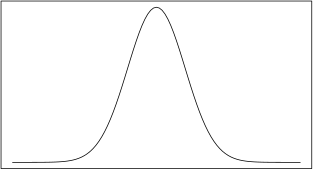
\includegraphics[scale=0.31]{fig/normal}
			\quad
			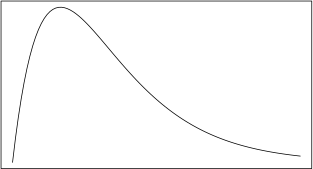
\includegraphics[scale=0.31]{fig/gamma}\\
			$\Downarrow$
		\end{center}
		\begin{center}	
			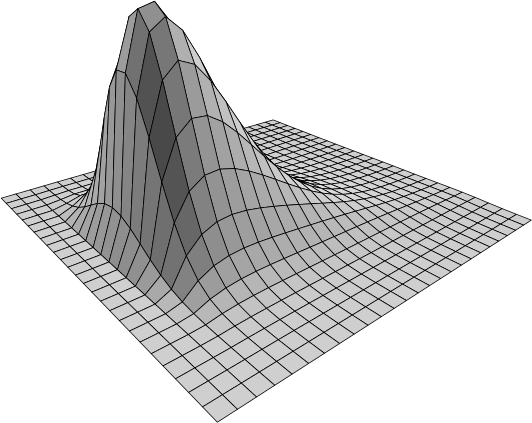
\includegraphics[scale=0.18]{fig/gumbel_cop}
		\end{center}
	\end{frame}
		
	\begin{frame}
		\frametitle{Copulas}
		\begin{itemize}
		\setlength\itemsep{2em}
		\item We can study the resulting multivariate distribution function to determine how efficacy and safety are correlated
		\item In practice, the form of the univariate distributions and the type of copula are unknown and must be estimated from the observed data
		\end{itemize}
	\end{frame}
		

	\begin{frame}
		\frametitle{Other joint modelling approaches} 
	\end{frame}	


	\begin{frame}
		\frametitle{Applications}
		\begin{itemize}
			\setlength\itemsep{2em}
			\item We can study the resulting multivariate distribution function to determine how efficacy and safety are correlated
			\item In practice, the form of the univariate distributions and the type of copula are unknown and must be estimated from the observed data
		\end{itemize}
	\end{frame}

\section{Joint Copula Models}

	\begin{frame}
		\frametitle{Definition}
		\begin{itemize}
			\setlength\itemsep{2em}
			\item foo
		\end{itemize}
	\end{frame}	


	\begin{frame}
		\frametitle{Copula concepts}
		\begin{itemize}
			\setlength\itemsep{2em}
			\item foo
		\end{itemize}
	\end{frame}	
	
	
	\begin{frame}
		\frametitle{Copula regression}
		\begin{itemize}
			\setlength\itemsep{2em}
			\item foo
		\end{itemize}
	\end{frame}	
		
	\begin{frame}
		\frametitle{Inference}
		\begin{itemize}
			\setlength\itemsep{2em}
			\item Principled method of combining prior beliefs with newly collected data 
			\item Provides a mechanism to incorporate information from animal models, previous studies, clinical expertise, etc.
			\item Simpler conceptual framework for adaptive designs
			\item Inference is based on posterior probabilities
		\end{itemize}
	\end{frame}	


	\begin{frame}
		\frametitle{Extensions}
		\begin{itemize}
			\setlength\itemsep{2em}
			\item foo
		\end{itemize}
	\end{frame}		
	
\section{Applications}
	
	\begin{frame}
		\frametitle{Dose-finding}
		Efficacy-Toxicity (EffTox)\footnote{Thall, P. and Cook, J. (2004), ``Dose-finding based on efficacy-toxicity trade-offs", Biometrics, 60:684-693.} is a study design which combines elements of Phase I and II trials
		\begin{itemize}
			\setlength\itemsep{1.5em}
		\item A Bayesian copula model for the probabilities of Efficacy and Toxicity as a function of dose
		\item Criteria for dose acceptability
        \item Trade-off contours quantifying the desirability of each dose
		\end{itemize}
	\end{frame}

	\begin{frame}
		\frametitle{Bayesian Copula model} 
		\begin{itemize}
			\setlength\itemsep{2em}
			\item Consider a binary bivariate outcome $Y=(Y_E,Y_T)$ where $Y_k \in \{0,1\},\,k=E,T$ 
			\item The marginal probability at dose $x_j$ for outcome $k$ is modelled as
			$\pi_{k,j}=\text{logit}^{-1}(\eta_{k,j})$ where $\eta_{k,j}$ is a linear function of dose
			\item The joint probability of both outcomes given dose and $\eta_{k,j}$ parameters $\theta$ is $Pr(Y_E=a,Y_T=b|x_j,\theta)=\pi(a,b|x_j,\theta)$ for $(a,b)=(1,1),(1,0),(0,1),(0,0)$
			
		\end{itemize}
	\end{frame}
	
	\begin{frame}
		\frametitle{Bayesian Copula model} 
		\begin{itemize}
			\setlength\itemsep{2em}
			\item The joint probability, $\pi(a,b|x_j,\theta)$, is modelled with a Farlie-Gumbel-Morgenstern (FGM) copula
			\item For subject $i$, let $(Y_{i,E},Y_{i,T})$ be the observed outcome and $x_{[i]}$ the assigned dose, the likelihood of the data $\mathcal{D}_n$ for all $n$ subjects is
			$\mathcal{L}(\mathcal{D}_n|\theta)=\prod_{i=1}^{n}\pi(Y_{i,E},Y_{i,T}|x_{[i]},\theta)$
			\item Finally, the posterior is $p(\theta|\mathcal{D}_n) \propto \mathcal{L}(\mathcal{D}_n|\theta) \times p(\theta)$
		\end{itemize}
	\end{frame}	
	
	\begin{frame}
		\frametitle{Dose Acceptability} 
		\begin{itemize}
			\setlength\itemsep{2em}
			\item Using information elicited from physicians, bounds are established to prevent assigning a dose which is likely to be ineffective or too toxic
			\item The trial is stopped if no dose is acceptable based on estimates from the Bayesian model 
		\end{itemize}
	\end{frame}
	
	\begin{frame}
		\frametitle{Trade-off contours} 
		\begin{columns}[T]
			\begin{column}{.5\textwidth}			
				\begin{itemize}
					\setlength\itemsep{1em}
					\item Trade-off contours represent equally desirable pairs of efficacy/toxicity probabilities (Prob(efficacy),Prob(toxicity))
					\item (0.5,0), (0.7,0.25), (1,0.6) equally desirable
					\item Dose desirability calculated from model estimates and used to assign dose in next cohort
				\end{itemize}
			\end{column}
			\begin{column}{.5\textwidth}
				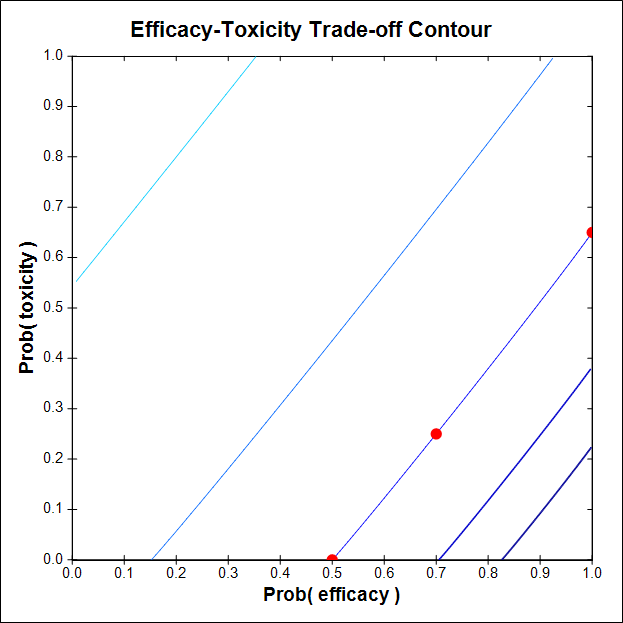
\includegraphics[height=5.8cm]{fig/image046}
			\end{column}
		\end{columns}		
	\end{frame}	


	
	\begin{frame}
		\frametitle{Benefit-Risk}
		\begin{itemize}
			\setlength\itemsep{1.5em}
			\item foo
		\end{itemize}
	\end{frame}

	\begin{frame}
		\frametitle{Other Applications}
		\begin{itemize}
			\setlength\itemsep{1.5em}
			\item foo
		\end{itemize}
	\end{frame}
	

\section{Future Research}

	\begin{frame}
		\begin{itemize}
			\setlength\itemsep{2em}
			\item How to elicit and incorporate non-standard prior distributions
			\item More flexible modelling of copula (copula conditional regression, nonparametric estimation)
			\item Implementation of more efficient, flexible, and easy to use software 
		\end{itemize}
		\begin{center}
		%	\includegraphics[scale=.55]{../fig/mod_comp1}		
		\end{center}
	\end{frame}

\section{Conclusion}

	\begin{frame}
		\begin{itemize}
			\setlength\itemsep{2em}
			\item Copula models
			\begin{itemize} 
				\item Use data more effectively
				\item Formally quantify risk-benefit tradeoff
			\end{itemize}
			\item Bayesian paradigm
			\begin{itemize}
			 \item Easier to interpret inference
			 \item More flexible designs
			 \end{itemize}
%			\item Improving study design reduces drug development time and makes trials more ethical and less costly
		\end{itemize}			
		\begin{center}
		%	\includegraphics[scale=.43]{../fig/misspec_plot1}
		\end{center}
	\end{frame}
	

\end{document} 